\documentclass[border=10pt]{standalone}

\usepackage{tikz}
\usepackage{tikzsymbols}
\usetikzlibrary{calc,patterns,shapes.geometric}

\def\centerarc[#1](#2)(#3:#4:#5){\draw[#1] ($(#2)+({#5*cos(#3)},{#5*sin(#3)})$) arc (#3:#4:#5);}

\begin{document}
	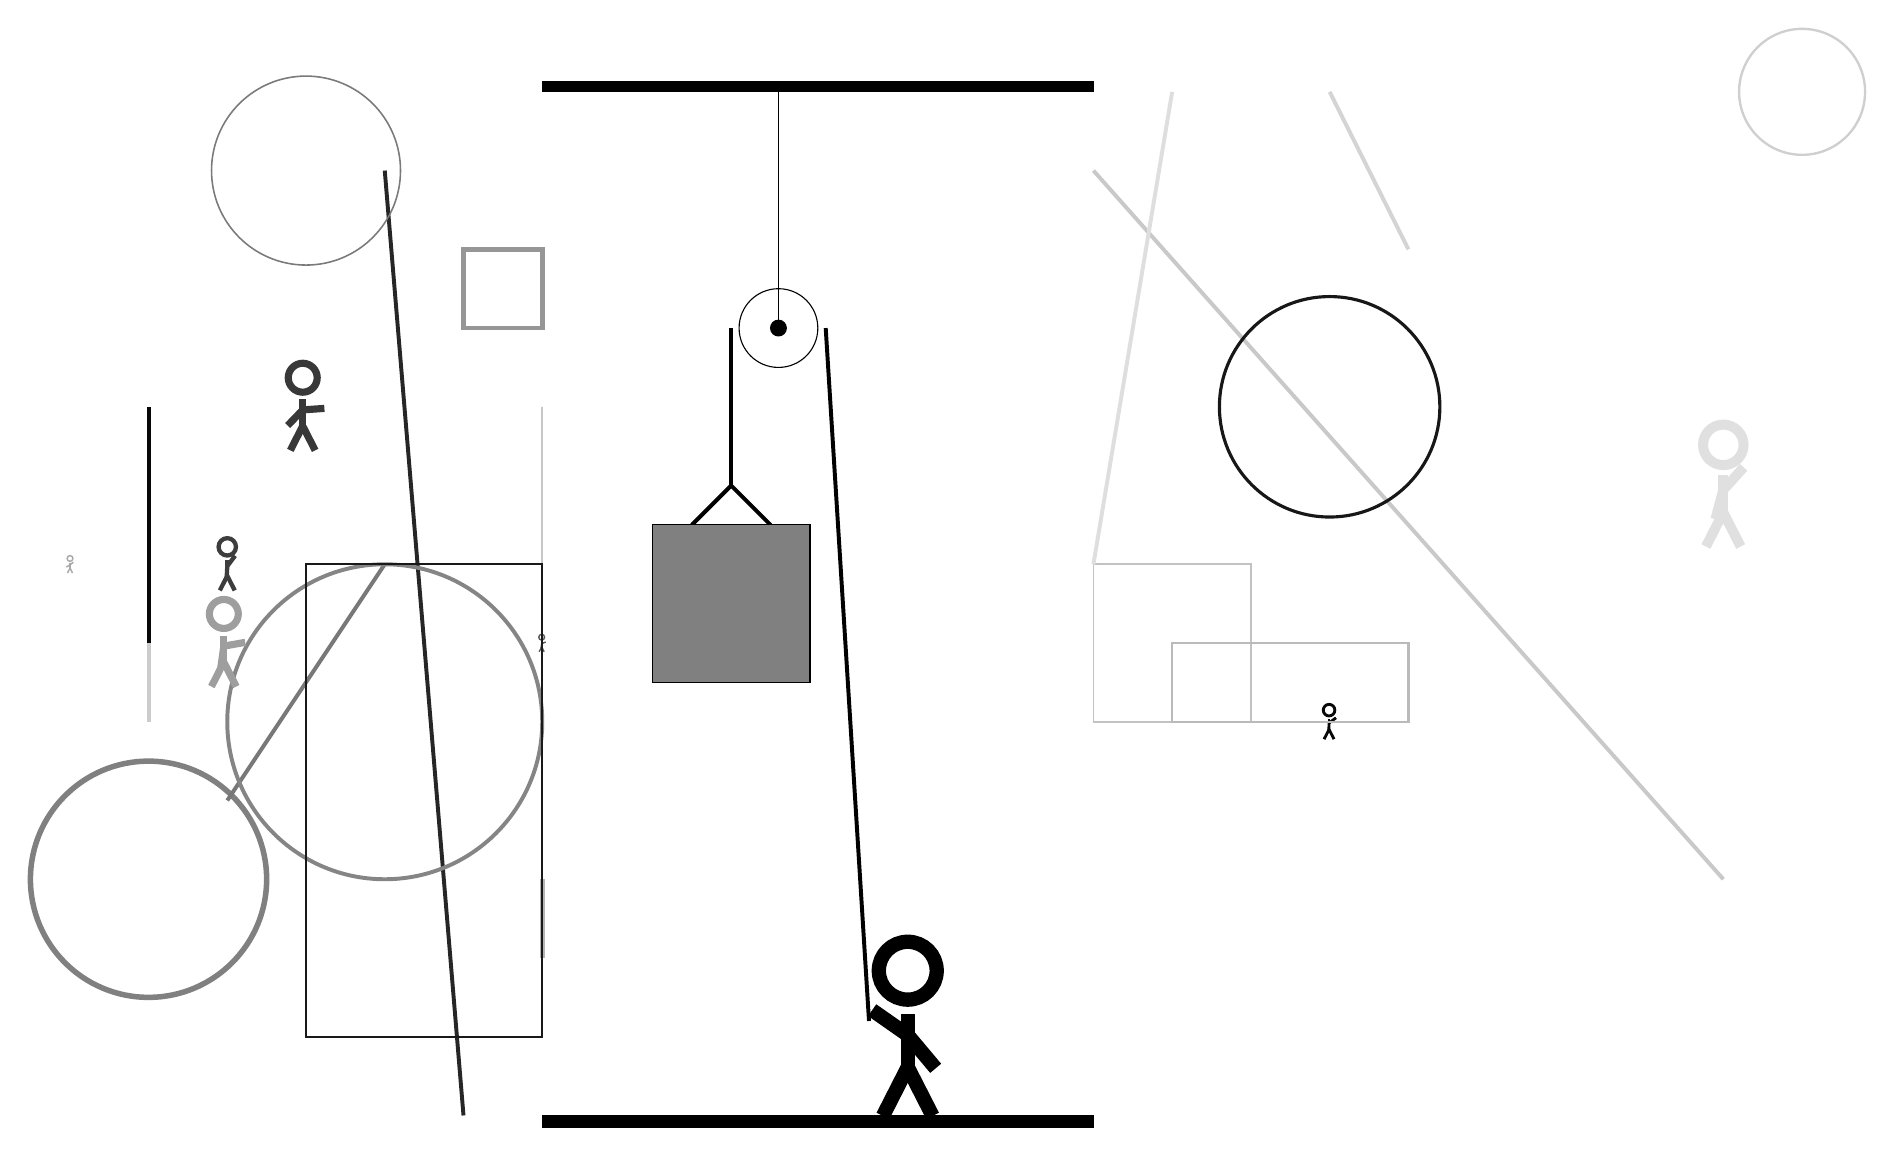
\begin{tikzpicture}
		%%%%% START %%%%%
		
		\draw[fill=black] (-2, 10) rectangle (5, 10.125);
		
		\draw (1, 7) circle (0.5);
		\draw[fill=black] (1, 7) circle (0.1);
		\draw (1, 10) -- (1, 7);
		
		\draw[line width=0.5mm] (-0.1, 4.5) -- (0.4, 5.0) -- (0.9, 4.5);
		\draw[fill=black!50] (-0.6, 4.5) rectangle (1.4, 2.5);
		
		\node[line width=0.3mm, color=black!97] at (8, 2) {\Strichmaxerl[2][88][37]};
		
		\node[line width=0.2mm, color=black!65] at (-2, 3) {\Strichmaxerl[1][83][22]};
		\draw[line width=0.2mm, color=black!24] (5, 4) rectangle (7, 2);
		\draw [line width=0.7mm, color=black!50](-7, 0) circle (1.5);
		
		\draw[line width=0.5mm, color=black!21](5, 9) -- (13, 0);
		
		\draw[line width=0.5mm, color=black!13](6, 10) -- (5, 4);
		\draw[line width=0.6mm, color=black!29] (-2, -1) rectangle (-2, 0);
		\draw [line width=0.3mm, color=black!19](14, 10) circle (0.8);
		\draw[line width=0.5mm, color=black!85](-3, -3) -- (-4, 9);
		\draw[line width=0.5mm, color=black!53](-4, 4) -- (-6, 1);
		\draw[line width=0.3mm, color=black!27] (6, 2) rectangle (9, 3);
		\node[line width=0.3mm, color=black!76] at (-6, 4) {\Strichmaxerl[3][87][53]};
		\draw[line width=0.2mm, color=black!22] (-2, 2) rectangle (-2, 6);
		\draw [line width=0.4mm, color=black!91](8, 6) circle (1.4);
		\node[line width=0.7mm, color=black!34] at (-8, 4) {\Strichmaxerl[1][30][40]};
		\draw[line width=0.5mm, color=black!97](-7, 3) -- (-7, 6);
		
		\draw [line width=0.5mm, color=black!48](-4, 2) circle (2.0);
		\draw[line width=0.5mm, color=black!20](-7, 3) -- (-7, 2);
		\draw[line width=0.5mm, color=black!17](9, 8) -- (8, 10);
		
		\node[line width=0.3mm, color=black!38] at (-6, 3) {\Strichmaxerl[5][82][10]};
		\node[line width=0.5mm, color=black!78] at (-5, 6) {\Strichmaxerl[5][46][4]};
		
		\draw[line width=0.3mm, color=black!90] (-2, -2) rectangle (-5, 4);
		\draw[line width=0.6mm, color=black!41] (-3, 7) rectangle (-2, 8);
		\node[line width=0.4mm, color=black!12] at (13, 5) {\Strichmaxerl[7][75][48]};
		\draw [line width=0.2mm, color=black!52](-5, 9) circle (1.2);
		
		\draw[line width=0.5mm] (0.4, 7) -- (0.4, 5.0);
		\centerarc[line width=0.5mm](1, 7)(0:180:0.6);
		\draw[line width=0.5mm](1.6, 7) -- (2.15, -1.8);
		
		\node at (2.6, -1.9) {\Strichmaxerl[10][-35][-50]};
		
		\draw[fill=black] (-2, -3) rectangle (5, -3.15);
		
		%%%%% END %%%%%
	\end{tikzpicture}
\end{document}